\documentclass[
  aps,
  prx,
  reprint,
  amsmath,
  amssymb,
  groupedaddress,
  nofootinbib,
  floatfix,
  longbibliography
]{revtex4-2}

\usepackage[T1]{fontenc}
\usepackage{microtype}
\usepackage{amsthm,mathtools,bm}
\usepackage{booktabs,array}
\usepackage{graphicx}
\usepackage{capt-of}
\usepackage{enumitem}
\usepackage{xcolor}
\usepackage[colorlinks=true,allcolors=blue!55!black]{hyperref}

\setlength{\textfloatsep}{9pt plus 2pt minus 2pt}
\setlength{\floatsep}{8pt plus 2pt minus 2pt}
\setlength{\intextsep}{8pt plus 2pt minus 2pt}
\renewcommand{\arraystretch}{1.08}
\newtheorem{proposition}{Proposition}
\newtheorem{remark}{Remark}
\newcommand{\QeFEM}{QeFEM}
\newcommand{\LQA}{LQA}
\newcommand{\FEM}{FEM}
\newcommand{\dSB}{dSB}
\newcommand{\Tr}{\operatorname{Tr}}
\newcommand{\sgn}{\operatorname{sign}}
\newcommand{\KL}{D_{\mathrm{KL}}}
\newcommand{\eps}{\varepsilon}

\begin{document}

\title{A Quantum-Inspired Annealing-Based Algorithm to solve Large-Scale Binary Optimization Problems}
\author{Ronit Dutta}
\affiliation{Singapore University of Technology and Design}
\author{Feng Pan}
\affiliation{Singapore University of Technology and Design}
\date{23 September 2026}

\begin{abstract}
Combinatorial optimization arises throughout science and industry, yet
finding good solutions becomes difficult as problem sizes grow and more complex. 
Many of these combinatorial problems (COPs), usually defined on graphs, can be 
written as quadratic unconstrained binary optimization (QUBO) hamiltonians, 
giving a common starting point for optimal configuration search. We introduce the 
quantum-enhanced free-energy machine (\QeFEM), a classical, quantum-inspired method 
that combines ideas from statistical physics, variational optimization, and annealing. 
It seeks to find the probabilistic thermal distribution of the graph vertices by mini
Gradient-based updates then guide
many candidate solutions in parallel toward feasible binary assignments.
We derive the method and analyze its search dynamics, then evaluate it on
MaxCut and planted Ising problems with different sizes and structures.
Across these demanding benchmarks, \QeFEM{} finds high-quality solutions
with a common solver framework. Recorded inputs, seeds, and settings
support repeatable experiments and controlled comparisons across CPUs
and accelerators.
\end{abstract}

\maketitle

\section{Introduction}
\label{sec:introduction}

Binary optimization asks for an assignment of finitely many decisions that
minimizes a cost or maximizes a reward. The variables may describe the two
sides of a graph cut, selected facilities, accepted constraints, or a spin
configuration. A common mathematical representation is quadratic
unconstrained binary optimization (QUBO); after an affine change of
variables, the same objective is an Ising energy. The representation is
general enough to encode many problems, but it does not remove their
combinatorial difficulty: $N$ unrestricted binary variables have $2^N$
possible assignments. MaxCut and general Ising optimization already contain
NP-hard cases \citep{karp1972,barahona1982,lucas2014}.

For MaxCut, the input is an undirected weighted graph $G=(V,E,w)$ and a
feasible solution is a partition $S\subseteq V$ of its vertices. The problem
is to find
\begin{equation}
 \max_{S\subseteq V}\; C(S),\qquad
 C(S)=\sum_{\{i,j\}\in E}w_{ij}
 \mathbf 1\{ |\{i,j\}\cap S|=1\}.
 \label{eq:maxcut-statement}
\end{equation}
Equivalently, a binary spin $s_i\in\{-1,+1\}$ marks each vertex's side of
the partition. In this paper, a reported MaxCut solution is such a binary
partition, scored with the original edge weights; the continuous QeFEM
state is the means of finding it.

Many useful solvers therefore exchange exhaustive enumeration for a search
over an easier auxiliary space. Simulated annealing explores binary states
stochastically \citep{kirkpatrick1983}. The free-energy machine (\FEM)
optimizes a factorized thermal distribution with gradients
\citep{shen2025}. Local quantum annealing (\LQA) instead optimizes a pure
product-state surrogate for a changing transverse-field Hamiltonian
\citep{bowles2022}. Discrete simulated bifurcation (\dSB) updates classical
position and momentum variables with a sign-dependent interaction
\citep{goto2021dsbm}. These algorithms differ in objective, dynamics, and
computational budget. Their common feature is that a continuous or
population-based search eventually returns an ordinary binary assignment.

\QeFEM{} places the search in a product of single-qubit mixed states. A
local state has a longitudinal component, which records the expected binary
decision; a transverse component, which couples to a driver; and an entropy,
which resists premature polarization. The objective is the mean-field free
energy of a transverse-field Ising model. We minimize it with classical
tensor operations and independently initialized replicas. The word
``quantum'' identifies the state family and the noncommuting driver in the
surrogate Hamiltonian. It does not imply entanglement, physical quantum
evolution, or quantum computational speedup.

The point of a detailed derivation is to identify precisely what this
relaxation can and cannot promise. The exact Gibbs state is generally
intractable, so the product ansatz introduces a substantial approximation.
The resulting free energy is nonconvex at low temperature. Annealing and
replica search can find strong states, but neither follows an adiabatic
theorem, and neither guarantees the optimal cut. Furthermore, the later
G-set experiments use a deliberately modified, discrete-neighbour search
direction. That update shares the state representation and final score with
the smooth method, but it is not the exact gradient of the original free
energy. Treating the two variants as identical would obscure both the
mathematics and the evidence.

The results require similar care. The main saved comparison consists of
frozen \QeFEM{} and \LQA{} configurations on K2000, Wishart, and Chook
instances. The G-set result combines historical attainment with a subsequent
adaptive search and fresh-seed confirmation. A separate FEM notebook
contains informative K2000 runs of \FEM{} and \dSB, but those runs are not
paired with the saved \QeFEM{} experiment in compute, numerical platform,
or seed protocol. We preserve these distinctions throughout rather than
compressing unlike measurements into one apparent league table.

This expanded manuscript is organized around four questions. First, how
does a binary Ising objective lead to the \QeFEM{} free energy? Second, what
do its stationary equations, gradients, and instability scale say about the
search dynamics? Third, what was actually run, including optimizer settings,
replica counts, seeds, and readout? Fourth, what do the stored endpoints
establish, and where does the method still fall short? The figures are
chosen to answer these questions directly: a winner trajectory and entropy
trace expose the annealing dynamics; population scaling diagnoses the K2000
plateau; instance-level curves show where planted error changes; and a
gap-before/after plot displays which revisited G-set graphs improved and
which supplied references were newly attained.

\section{From binary objectives to an annealed variational problem}
\label{sec:formulation}

\subsection{QUBO, Ising variables, and MaxCut}

Let $\bm x\in\{0,1\}^{N}$ and let $Q=Q^{\mathsf T}$ be a real matrix. We
write a QUBO as
\begin{equation}
 E_Q(\bm x)=\bm x^{\mathsf T}Q\bm x+c.
 \label{eq:qubo}
\end{equation}
The symmetric convention is explicit: off-diagonal entries of $Q$ occur
twice in the matrix product. Define $s_i=1-2x_i$, so that
$x_i=(1-s_i)/2$ and $s_i\in\{-1,+1\}$. Direct substitution gives
\begin{align}
 E_Q(\bm s)
 &=c+\frac14(\bm 1-\bm s)^{\mathsf T}
                 Q(\bm 1-\bm s)\nonumber\\
 &=c+\frac14\bm 1^{\mathsf T}Q\bm 1
   -\frac12(Q\bm 1)^{\mathsf T}\bm s
   +\frac14\bm s^{\mathsf T}Q\bm s.
 \label{eq:qubo-expand}
\end{align}
Since $s_i^2=1$, the diagonal part of the last term is constant. With
each unordered pair counted once,
\begin{align}
 E_I(\bm s)&=c_0+\sum_i h_i s_i+\sum_{i<j}K_{ij}s_i s_j,
 \label{eq:ising-energy}\\
 c_0&=c+\tfrac14\bm 1^{\mathsf T}Q\bm 1+\tfrac14\Tr Q,
 \nonumber\\
 h_i&=-\tfrac12(Q\bm 1)_i,
 \quad K_{ij}=\tfrac12Q_{ij}\quad(i\ne j).
 \label{eq:qubo-map}
\end{align}
The choice $s_i=2x_i-1$ reverses the sign of $h_i$ but is otherwise
equivalent. Writing the affine map matters when results from two software
packages are compared; a silent sign or factor-of-two change can alter a
reported energy while leaving the spin vector unchanged.

For the MaxCut problem in Eq.~\eqref{eq:maxcut-statement}, encode a
partition by $s_i=+1$ on $S$ and $s_i=-1$ otherwise. The edge indicator
then becomes $(1-s_i s_j)/2$, giving
\begin{equation}
 C(\bm s)=\sum_{\{i,j\}\in E}w_{ij}\frac{1-s_i s_j}{2}
 =\frac{W-E_G(\bm s)}{2},
 \label{eq:cut}
\end{equation}
where $W=\sum_{\{i,j\}\in E}w_{ij}$ and
$E_G(\bm s)=\sum_{\{i,j\}\in E}w_{ij}s_i s_j$.
This identity holds for signed weights as well as nonnegative ones. We
use $E_G$ as the Ising energy to be minimized in the graph experiments.
If $K$ is its symmetric zero-diagonal coupling matrix, then
$E_G(\bm s)=\tfrac12\bm s^{\mathsf T}K\bm s$.
For K2000, the final cut is always recomputed with the original unscaled
edge weights, not inferred from the value of the relaxed objective.

\subsection{A transverse-field Gibbs target}

Replace each classical spin $s_i$ by the Pauli operator $Z_i$ to form the
diagonal problem Hamiltonian
\begin{equation}
 H_P=c_0 I+\sum_i h_i Z_i+\sum_{i<j}K_{ij}Z_iZ_j.
 \label{eq:hp}
\end{equation}
Its computational-basis eigenvalues are precisely the Ising costs. We
introduce a transverse driver with strength $\Gamma\geq0$,
\begin{equation}
 H_{\Gamma}=H_P-\Gamma\sum_i X_i.
 \label{eq:hgamma}
\end{equation}
At a temperature $T>0$, the corresponding exact Gibbs state is
\begin{equation}
 \sigma_{T,\Gamma}
 =\frac{e^{-H_{\Gamma}/T}}{Z_{T,\Gamma}},
 \qquad Z_{T,\Gamma}=\Tr e^{-H_{\Gamma}/T}.
 \label{eq:gibbs}
\end{equation}
The state has a $2^N\times2^N$ matrix representation and is never formed
by the algorithm. Its role is variational: it identifies an objective whose
terms have a controlled thermodynamic origin. The schedule changes this
objective over optimization steps. It is not a physical time evolution of
Eq.~\eqref{eq:hgamma}.

For any density matrix $\rho$, the quantum relative entropy is
$\KL(\rho\Vert\sigma)=\Tr[\rho(\log\rho-\log\sigma)]$. Since
$\log\sigma_{T,\Gamma}=-H_\Gamma/T-\log Z_{T,\Gamma}$,
\begin{align}
 T\KL(\rho\Vert\sigma_{T,\Gamma})
 &=\Tr(\rho H_\Gamma)-T S(\rho)
   +T\log Z_{T,\Gamma}\nonumber\\
 &=\mathcal F_{T,\Gamma}(\rho)-F^*_{T,\Gamma},
 \label{eq:klidentity}
\end{align}
where $S(\rho)=-\Tr(\rho\log\rho)$,
$\mathcal F_{T,\Gamma}(\rho)=\Tr(\rho H_\Gamma)-T S(\rho)$,
and $F^*_{T,\Gamma}=-T\log Z_{T,\Gamma}$. Positivity of relative entropy
implies $\mathcal F_{T,\Gamma}(\rho)\geq F^*_{T,\Gamma}$, with equality at
the exact Gibbs state. Restricting $\rho$ to an inexpensive family converts
this identity into a tractable variational approximation
\citep{nielsen2010,wainwright2008}. It does not make the restricted minimum
equal to the exact free energy.

\subsection{Product states and the Bloch disk}

\QeFEM{} restricts the trial state to
\begin{equation}
 \begin{aligned}
 \rho&=\bigotimes_{i=1}^{N}\rho_i,\\
 \rho_i&=\tfrac12\bigl(I+m_{x,i}X_i+m_{z,i}Z_i\bigr),\\
 &m_{x,i}^2+m_{z,i}^2\leq1.
 \end{aligned}
 \label{eq:ansatz}
\end{equation}
No intersite entanglement or classical correlation is represented in this
family. The restriction to the $x$--$z$ Bloch disk is sufficient for
minimizing the product-state free energy of the real Hamiltonian
Eq.~\eqref{eq:hgamma}. Indeed, $H_\Gamma$ contains no $Y_i$ expectation,
while the local entropy decreases as the Bloch length increases. Given any
site with a nonzero $y$ component, setting that component to zero preserves
the energy and weakly increases the entropy. It therefore cannot increase
$\mathcal F_{T,\Gamma}$. The two-coordinate ansatz is a consequence of the
chosen Hamiltonian, not an arbitrary truncation of a needed $y$ degree of
freedom.

Let $R_i=\sqrt{m_{x,i}^2+m_{z,i}^2}$. The eigenvalues of $\rho_i$ are
$(1\pm R_i)/2$, so its entropy is the binary entropy of those eigenvalues:
\begin{equation}
 S_i= -\frac{1+R_i}{2}\log\frac{1+R_i}{2}
      -\frac{1-R_i}{2}\log\frac{1-R_i}{2}.
 \label{eq:entropy}
\end{equation}
The full entropy is additive, $S(\rho)=\sum_iS_i$. Its maximum is
$N\log2$, attained at the maximally mixed product state. In contrast,
$S_i\to0$ as $R_i\to1$.

For a product state,
$\langle Z_i\rangle=m_{z,i}$ and
$\langle Z_iZ_j\rangle=m_{z,i}m_{z,j}$ for $i\ne j$.
Consequently the restricted free energy is
\begin{equation}
 \boxed{\begin{aligned}
 \mathcal F_{T,\Gamma}(\bm m_x,\bm m_z)
 &=c_0+\sum_i h_i m_{z,i}
   +\sum_{i<j}K_{ij}m_{z,i}m_{z,j}\\
 &\quad-\Gamma\sum_i m_{x,i}-T\sum_iS_i.
 \end{aligned}}
 \label{eq:qefemF}
\end{equation}
This is the smooth \QeFEM{} objective. The first line is the exact energy
expectation \emph{within the product ansatz}; factorization of pair
expectations is the approximation to the exact Gibbs state. The transverse
term rewards positive $x$ polarization, and the entropy term favors local
mixture at high temperature. The constant $c_0$ affects reported energies
but not the variational minimizer.

The longitudinal component also has a direct probabilistic interpretation.
A $Z_i$ measurement returns $s_i\in\{-1,+1\}$ with probability
\begin{equation}
 q_i(s_i)=\frac{1+s_i m_{z,i}}{2},\qquad
 q(\bm s)=\prod_iq_i(s_i).
 \label{eq:measure}
\end{equation}
This distribution is a useful interpretation of the state; the benchmark
solver does not sample it for final scoring. It uses deterministic sign
readout after optimization, as specified in Sec.~\ref{sec:algorithm}.

\section{Stationary structure and annealing dynamics}
\label{sec:theory}

\subsection{Unconstrained fields and exact local derivatives}

Directly optimizing $(m_x,m_z)$ would require projection back into the
Bloch disk. Instead, each site has unconstrained real fields
$\bm a_i=(u_i,v_i)^{\mathsf T}$ and radius
$r_i=\sqrt{u_i^2+v_i^2}$. Define
\begin{equation}
 \begin{aligned}
 \bm m_i&=(m_{x,i},m_{z,i})^{\mathsf T}
 =g(r_i)\bm a_i,\\
 g(r)&=\begin{cases}\tanh r/r,&r>0,\\1,&r=0.\end{cases}
 \end{aligned}
 \label{eq:fieldmap}
\end{equation}
Then $R_i=\tanh r_i<1$ for finite fields, so positivity of every local
density matrix is automatic. More explicitly,
\begin{equation}
 \rho_i=\frac{e^{u_iX_i+v_iZ_i}}{2\cosh r_i},
 \label{eq:localexp}
\end{equation}
because $(u_iX_i+v_iZ_i)^2=r_i^2I$.
Equation~\eqref{eq:fieldmap} is therefore an exponential-family
parameterization of the open Bloch disk. At $r_i=0$, it is interpreted by
continuity rather than evaluated as $0/0$.

The local entropy is especially stable in these coordinates:
\begin{equation}
 S_i=\log(2\cosh r_i)-r_i\tanh r_i.
 \label{eq:fieldentropy}
\end{equation}
The implementation evaluates the log-cosh term by a stable log-sum-exp
operation to avoid overflow. Differentiating
Eq.~\eqref{eq:fieldmap} gives the symmetric Jacobian
\begin{equation}
 \begin{aligned}
 J_i&=\frac{\partial\bm m_i}{\partial\bm a_i}
 =g(r_i)I+\frac{g'(r_i)}{r_i}\bm a_i\bm a_i^{\mathsf T},\\
 g'(r)&=\frac{r\,\operatorname{sech}^2r-\tanh r}{r^2}.
 \end{aligned}
 \label{eq:jacobian}
\end{equation}
Its tangential eigenvalue is $\tanh r/r$, and its radial eigenvalue is
$\operatorname{sech}^2r$. Both are positive at finite $r$; both tend to one
as $r\to0$. The radial eigenvalue becomes small when the local state is
nearly pure, an explicit reason that field-space optimization can slow near
the boundary even while the physical-coordinate gradient remains large.

Define the instantaneous longitudinal effective field
\begin{equation}
 H_i(\bm m_z)=h_i+\sum_{j\ne i}K_{ij}m_{z,j}.
 \label{eq:effectivefield}
\end{equation}
Because $dS_i/dR_i=-\operatorname{arctanh}R_i$,
\begin{align}
 \frac{\partial\mathcal F}{\partial m_{x,i}}
 &=-\Gamma+T\frac{\operatorname{arctanh}R_i}{R_i}m_{x,i},
 \label{eq:gradx}\\
 \frac{\partial\mathcal F}{\partial m_{z,i}}
 &=H_i+T\frac{\operatorname{arctanh}R_i}{R_i}m_{z,i}.
 \label{eq:gradz}
\end{align}
The quotient tends to one as $R_i\to0$. Since
$\operatorname{arctanh}R_i=r_i$ and
$\bm m_i/R_i=\bm a_i/r_i$, the two physical-coordinate
gradients form the remarkably simple vector
\begin{equation}
 \nabla_{\bm m_i}\mathcal F
 =\binom{-\Gamma}{H_i}+T\bm a_i.
 \label{eq:physicalgrad}
\end{equation}
Thus the exact gradient seen by the optimizer is
\begin{equation}
 \boxed{\nabla_{\bm a_i}\mathcal F
 =J_i\binom{-\Gamma}{H_i}
  +T\operatorname{sech}^2(r_i)\bm a_i.}
 \label{eq:fieldgrad}
\end{equation}
The second term follows from $J_i\bm a_i=\operatorname{sech}^2(r_i)\bm a_i$.
This expression agrees with automatic differentiation of
Eq.~\eqref{eq:qefemF}; Appendix~\ref{app:derivations} shows the chain rule
in detail. Exact manual evaluation is an implementation choice, whereas
changing $H_i$ changes the vector field being optimized.

\subsection{Self-consistency and the classical endpoint}

At any finite $r_i$, $J_i$ is invertible. A stationary point therefore
satisfies $\nabla_{\bm m_i}\mathcal F=0$, giving
\begin{equation}
 u_i=\frac{\Gamma}{T},
 \qquad v_i=-\frac{H_i(\bm m_z)}{T}.
 \label{eq:stationaryfields}
\end{equation}
Substitution into the Bloch map yields the product-state self-consistency
equation
\begin{equation}
 m_{z,i}=-\frac{H_i}{\sqrt{\Gamma^2+H_i^2}}
     \tanh\!\left(\frac{\sqrt{\Gamma^2+H_i^2}}{T}\right),
 \label{eq:selfconsistency}
\end{equation}
with the continuous zero-field limit understood. The transverse component is
\begin{equation}
 m_{x,i}=\frac{\Gamma}{\sqrt{\Gamma^2+H_i^2}}
 \tanh\!\left(\frac{\sqrt{\Gamma^2+H_i^2}}{T}\right).
 \label{eq:selfconsistency-x}
\end{equation}
These are coupled equations: changing one site's $m_z$ changes the fields
of its neighbors. Their multiple solutions at low temperature are one
manifestation of the nonconvex landscape. The optimizer does not solve
Eq.~\eqref{eq:selfconsistency} by fixed-point iteration; its annealed
gradient updates need not be at equilibrium at any intermediate step.

If $\Gamma=0$ while $T>0$, Eq.~\eqref{eq:selfconsistency} reduces to the
classical mean-field equation
\begin{equation}
 m_{z,i}=-\tanh\!\left(\frac{H_i}{T}\right),
 \qquad m_{x,i}=0.
 \label{eq:classicalmf}
\end{equation}
At $T\to0$ and $\Gamma\to0$, strongly nonzero local fields drive
$|m_z|\to1$. This limiting statement is local and conditional. Finite
optimizer runs can retain uncertain sites or become trapped in suboptimal
sign patterns. If $T\to0$ at fixed $\Gamma>0$, the transverse component
need not disappear; removing the driver is essential to the intended
classical endpoint.

\begin{proposition}[Relation to the classical FEM family]
At $\Gamma=0$, the minimum of Eq.~\eqref{eq:qefemF} over the product-state
Bloch disks equals its minimum over the subfamily $m_{x,i}=0$ for every
site. Hence the transverse state coordinate does not improve the optimal
\emph{static} classical mean-field free energy at the endpoint.
\end{proposition}
\begin{proof}
For fixed $m_{z,i}$, the problem energy is independent of $m_{x,i}$.
Setting $m_{x,i}=0$ decreases $R_i$ and weakly increases the entropy
$S_i$, because $S_i$ is decreasing in $R_i$. At $\Gamma=0$, the driver term
vanishes. The change therefore weakly decreases the free energy at every
site. Applying it to an arbitrary product state proves the claim.
\end{proof}

This fact resolves an apparent paradox in method comparisons. A transverse
coordinate can change the \emph{path} through which a basin is entered, but
it does not imply a theorem that \QeFEM{} must defeat an optimized classical
\FEM{} run on every instance. The practical algorithms also use different
parameterizations, schedules, normalizations, and optimizers. Their endpoint
quality is an empirical question.

\subsection{A curvature scale for the onset of polarization}

The zero-field case $h_i=0$ admits a particularly informative local
analysis. The unpolarized longitudinal state $\bm m_z=0$ has
$m_x=\tanh(\Gamma/T)$ at a stationary point. Let $\lambda_{\min}(K)$
be the smallest eigenvalue of the symmetric coupling matrix, and write
$\kappa=-\lambda_{\min}(K)$ when this eigenvalue is negative. The
longitudinal Hessian at that state is
\begin{equation}
 \nabla^2_{\bm m_z}\mathcal F\big|_{\bm m_z=0}
 =K+q(T,\Gamma)I,
 \qquad
 q(T,\Gamma)=\frac{\Gamma}{\tanh(\Gamma/T)},
 \label{eq:stability}
\end{equation}
where $q(T,0)=T$ by continuity. To see the local term, use
$\operatorname{arctanh}R/R$ in Eq.~\eqref{eq:gradz} at
$R=\tanh(\Gamma/T)$: it becomes
$(\Gamma/T)/\tanh(\Gamma/T)$ and is multiplied by $T$.
The first unstable longitudinal mode appears when
$q(T,\Gamma)$ falls through $\kappa$. If $q>\kappa$, all longitudinal
eigenmodes have positive curvature at this stationary state; if
$q<\kappa$, at least one has negative curvature.

This criterion explains the later G-set spectral schedules. They
parameterize a desired $q$ relative to the graph-specific $\kappa$, rather
than cooling solely according to an absolute temperature that has a
different meaning on each weighted graph. Defining
$\rho=\Gamma/T$, one can recover physical schedule values from $q$ and
$\rho$:
\begin{equation}
 T=q\frac{\tanh\rho}{\rho},
 \qquad \Gamma=q\tanh\rho,
 \label{eq:spectralinvert}
\end{equation}
with $T=q$ when $\rho=0$. A schedule that lowers $q/\kappa$ from above
one to below one moves through the local polarization threshold. This
is a statement about curvature around one stationary state, not a proof
that the ensuing trajectory finds the ground state.

At sufficiently high temperature there is also a useful global statement.
The Hessian of $-S_i$ in physical Bloch coordinates has radial eigenvalue
$1/(1-R_i^2)$ and tangential eigenvalue
$\operatorname{arctanh}(R_i)/R_i$; both are at least one. Thus the entropy
contributes at least $T I$ to the physical-coordinate Hessian. If
$T>\kappa$, Eq.~\eqref{eq:qefemF} is strictly convex over the product of
open Bloch disks, even in the presence of the linear transverse driver.
The local condition $q>\kappa$ may hold at lower $T$ and is weaker than
this sufficient global-convexity bound. These results clarify why an
initial high-temperature phase can be easy to optimize and why a later
cooling phase can acquire many competing basins.

\subsection{What the discrete-neighbour continuation changes}

The current smooth K2000, Wishart, and Chook runs use the exact gradient of
Eq.~\eqref{eq:qefemF}. A later G-set search additionally studies a
surrogate direction. At update $t$, define
\begin{equation}
 \widetilde{\bm m}_z^{(t)}
 =(1-\lambda_t)\bm m_z^{(t)}
   +\lambda_t\sgn(\bm m_z^{(t)}),
 \qquad 0\leq\lambda_t\leq1.
 \label{eq:discretenbr}
\end{equation}
The term $K\bm m_z$ in the longitudinal field of
Eq.~\eqref{eq:fieldgrad} is replaced by
$K\widetilde{\bm m}_z^{(t)}$; the local Bloch Jacobian, transverse term,
and entropy derivative remain continuous. At $\lambda_t=0$ this is the
exact smooth gradient. A gradual schedule or a hard switch can increase
$\lambda_t$ during the run. When $\lambda_t>0$, the resulting vector is
generally \emph{not} the gradient of the original free energy, so
monotone descent of Eq.~\eqref{eq:qefemF} is not promised. Final binary
assignments are nevertheless scored with the original couplings.
The G-set results that use this update must therefore be described as a
distinct search variant. The frozen K2000 experiment has not applied it.

\section{Numerical algorithm and what a trajectory means}
\label{sec:algorithm}

\subsection{Coupling scale and the implemented objective}

All evaluated instances have zero local fields. Let $K^{\rm raw}$ be the
symmetric, zero-diagonal Ising coupling matrix. For a graph with edges
listed once, the implementation defines
\begin{equation}
 \begin{aligned}
 c_K&=\sqrt{\frac{1}{N}\sum_{i,j}(K^{\rm raw}_{ij})^2}\\
    &=\sqrt{\frac{2}{N}\sum_{\{i,j\}\in E}w_{ij}^2},
 \qquad K=K^{\rm raw}/c_K.
 \end{aligned}
 \label{eq:rmscoupling}
\end{equation}
It optimizes Eq.~\eqref{eq:qefemF} with $K$, then scores binary spins
against $K^{\rm raw}$. The numerical values of $T$ and $\Gamma$ must
therefore be read in units of the normalized interaction scale. If one
multiplies the normalized free energy by $c_K$, the equivalent physical
temperature and transverse field are $c_KT$ and $c_K\Gamma$. Coupling
normalization is more than a harmless change of printed units if the
temperature and driver schedules are left fixed while $c_K$ changes.

The selected scale is 44.71018 for K2000, 0.316598 for the saved Wishart
instances, and 3.162278 for the saved Chook instances. The values and
their source configurations are retained with the result folders. G-set
uses graph-specific normalization, and the later spectral schedule also
uses the lowest eigenvalue of the normalized graph matrix.

\subsection{Initialization, schedules, and optimization}

A trial starts with $B$ independent replicas. For replica $b$ and site $i$,
the two local fields are initialized as
\begin{equation}
 a^{(0)}_{b,i,d}=h_{\rm init}\,\xi_{b,i,d},
 \qquad \xi_{b,i,d}\sim\mathcal N(0,1),\quad d\in\{x,z\}.
 \label{eq:init}
\end{equation}
An isolated CPU random generator produces the stored initialization for
each seed before it is transferred to the compute device. This improves
replayability; it does not make distinct devices bitwise equivalent.
The K2000 $h_{\rm init}$ is 0.1. A trial is one full population of $B$
replicas, not one replica.

For $L$ optimizer updates, define $\tau_t=t/(L-1)$ for
$t=0,\ldots,L-1$. The simple frozen schedules have
\begin{align}
 T_t&=T_{\min}+(T_{\max}-T_{\min})(1-\tau_t),
 \label{eq:tempcurve}\\
 \Gamma_t&=\Gamma_{\min}+
 (\Gamma_{\max}-\Gamma_{\min})
 \left[1-\min\!\left(\frac{\tau_t}{f_\Gamma},1\right)\right].
 \label{eq:gammacurve}
\end{align}
The code passes the reciprocal $\beta_t=1/T_t$ to the free-energy
kernel. For K2000 and Wishart, $f_\Gamma=0.5$, so the transverse field
vanishes halfway and the remaining updates optimize with $\Gamma=0$.
For Chook, $f_\Gamma=1$. The G-set runs also use quadratic cooling or the
spectral construction of Eq.~\eqref{eq:spectralinvert}, according to their
graph-level plans. A schedule is applied to the objective at each update;
it is not a simulated measurement history or Schr\"odinger evolution.

For the frozen K2000, Wishart, and Chook runs, automatic differentiation
computes Eq.~\eqref{eq:fieldgrad}, and PyTorch RMSprop updates all field
coordinates. The recorded implementation uses ordinary \emph{coupled}
weight decay, so its elementwise updates can be written as
\begin{align}
 \widetilde g_t&=\nabla_{\bm a}\mathcal F_t+\lambda_{\rm wd}\bm a_t,
 &v_t&=\alpha v_{t-1}+(1-\alpha)\widetilde g_t^{\odot2},
 \label{eq:rmsprop1}\\
 b_t&=\mu b_{t-1}+\frac{\widetilde g_t}{\sqrt{v_t}+\eps_{\rm opt}},
 &\bm a_{t+1}&=\bm a_t-\eta b_t.
 \label{eq:rmsprop2}
\end{align}
These equations describe the non-centered, non-Nesterov mode used in the
saved plan. The operations are elementwise in the optimizer state, except
for the matrix product in the gradient. Here
$\eps_{\rm opt}=10^{-8}$. Weight decay changes the numerical trajectory
and thus must be reported with the learning rate and momentum.
Because each replica has separate coordinates, the batch is a parallel
collection of independent optimizations under the same graph and schedule.
The implementation backpropagates a sum of per-replica free energies; it
does not divide the gradient by $B$.

For clarity, the complete frozen-run logic is:
\begin{enumerate}[label=\arabic*.,leftmargin=2em]
 \item Load and validate the graph or planted Ising instance; form normalized
       couplings $K=K^{\rm raw}/c_K$.
 \item For each declared seed, construct $B\times N\times2$ Gaussian
       initial fields and arrays $\{T_t,\Gamma_t\}_{t=0}^{L-1}$.
 \item For every update, map fields through Eq.~\eqref{eq:fieldmap},
       evaluate Eq.~\eqref{eq:qefemF}, and apply Eq.~\eqref{eq:rmsprop1}
       --\eqref{eq:rmsprop2} or the declared alternative optimizer.
 \item After exactly $L$ updates, decode all $B$ final states and rescore
       each binary vector with the raw instance objective.
 \item Record the best final replica for that seed; aggregate these trial
       endpoints using the declared mean, best, gap, and exact-hit metrics.
\end{enumerate}
The K2000 population experiment uses nested prefixes of the same initialized
8,192-replica population for each seed. This controls the random population
when $B$ changes: a 128-replica run uses exactly the first 128 initial
states of that seed's 8,192-replica run, and similarly for larger sizes.
It does not imply that their later trajectories remain prefixes, since
floating-point batching and optimizer execution can differ.

\subsection{Binary readout and scoring}

The implemented final readout is
\begin{equation}
 \widehat s_{b,i}=\begin{cases}+1,&m^{(L)}_{z,b,i}>0,\\-1,&m^{(L)}_{z,b,i}\leq0.
 \end{cases}
 \label{eq:readout}
\end{equation}
This is equivalent to rounding the probability
$p_{b,i}=(1+m_{z,b,i})/2$ as used by the solver, including the tie at
$p=1/2$. It yields a feasible binary vector for every replica. For
MaxCut, we evaluate Eq.~\eqref{eq:cut}; for planted Ising instances we
evaluate $E_I(\widehat{\bm s}_b)$ and compare it with the supplied planted
energy. No local improvement, bit flipping, coordinate splicing, or
selection of an intermediate iterate is part of the frozen endpoint
protocol.

This distinction is crucial for interpreting trajectory figures. The
stored K2000 trace first selects the final best replica of the best
endpoint trial, then replays that \emph{same replica} from its initial
field to the final update. The curve is not the maximum cut over the
population at every step. Its temporary decreases are possible and do
not contradict final best-of-population selection. The entropy trace is
likewise the sum of site entropies for that coherent replica, divided by
$N$ when plotted.

\subsection{Arithmetic and storage}

For a dense graph, one longitudinal field evaluation is a batched
matrix product $\bm m_zK$, costing $O(BN^2)$ arithmetic, with
$O(N^2+BN)$ persistent storage before optimizer buffers and temporary
autograd tensors. An edge-list or sparse matrix contraction can reduce
arithmetic to $O(B|E|+BN)$ and graph storage to $O(|E|)$, subject to device
support and implementation details. K2000 is complete, so $|E|=N(N-1)/2$
and the dense formulation is natural. Large replica counts improve the
number of basins explored but increase memory and arithmetic nearly
linearly in $B$. Hence solution quality at $B=8{,}192$ cannot be read as
the quality of a single cheap trajectory, and unmatched wall-clock
measurements across methods are not evidence of a speedup.

\section{Experimental material and evaluation protocol}
\label{sec:experiments}

\subsection{Instance families and reference values}

The saved evidence covers two MaxCut families and two planted Ising
families. G-set
G1--G54 consists of 54 MaxCut graphs with varied size and topology; the
supplied target file serves as the versioned cut reference
\citep{yeGset}. K2000 is a complete signed 2,000-vertex graph with
$2{,}000\times1{,}999/2=1{,}999{,}000$ undirected edges
\citep{inagaki2016science}. Its stored target cut is 33,337. A stored
target is a known-quality comparison value, not in itself a certificate of
global optimality.

\subsection{Planted data and their construction}

The Wishart bank contains one dense 500-spin instance at each
$\alpha=M/N\in\{0.1,0.2,\ldots,1.0\}$, with $M=50,100,\ldots,500$.
Its generator centers $M$ Gaussian columns to make them orthogonal to a
planted spin direction, forms a zero-diagonal coupling matrix from their
Gram matrix, and applies a random spin gauge \citep{hamze2020}. The Chook
bank instead contains one sparse, periodic $32\times32$ lattice at each
requested $p(C_3)\in\{0.0,0.1,\ldots,1.0\}$. Edge-disjoint local tiles
are drawn from the $C_2/C_3$ mixture so that a common planted spin
assignment minimizes their sum; a gauge hides that assignment
\citep{perera2020}. Each saved file carries its planted spins and energy.
These are fixed local realizations of the published families, not the
unpublished matrices used in the cited figures; each plotted parameter
point describes one file rather than an ensemble average.

\subsection{Scoring and endpoint interpretation}

For a MaxCut candidate, the recorded residual is
\begin{equation}
 \Delta_C=C_{\rm ref}-C(\widehat{\bm s}).
 \label{eq:cutgap}
\end{equation}
If $\Delta_C=0$, the stored reference was attained. If a new cut exceeded
it, the residual would be negative; none of the retained G-set results
exceeded its supplied references. For planted instances, the recorded
energy excess and relative error are
\begin{equation}
 \Delta_E=E(\widehat{\bm s})-E_0,
 \qquad
 \eps=\frac{|E(\widehat{\bm s})-E_0|}{|E_0|}.
 \label{eq:plantedmetric}
\end{equation}
An exact hit means the final rescored energy equals the supplied planted
energy within the stored benchmark's exact scoring convention. A hit
\emph{trial} means at least one replica in that trial hits. The number of
such trials must not be confused with the number of hitting replicas;
the available compact paper records preserve the winning endpoint and
trial hit status, not every candidate population for every benchmark.

\subsection{Frozen \QeFEM{} and \LQA{} comparison}

The K2000, Wishart, and Chook experiments use selected, frozen
family-level configurations from the portable \texttt{qefem\_prof}
recheck plans. They were chosen after exploratory tuning and therefore
should be interpreted as evaluations of tuned procedures on the stored
instances, not as a pristine held-out generalization study. Every
\QeFEM{} trial evolves 8,192 replicas for the canonical comparison. The
K2000 and Wishart experiments use five seeded trials per instance; Chook
combines two predeclared five-seed batches for ten trials per instance.
The CPU, float32 portable evaluation is recorded with source revision
\texttt{b14f73c53305b55242b418ef2013fba0ac3cce54} and input hashes.

\begin{table*}[t]
\centering\small
\caption{Frozen \QeFEM{} schedules and budgets. A trial includes all
replicas. The driver reaches zero at fraction $f_\Gamma$ of the run.
Temperature follows a linear decrease in $T$, not a linear increase in
$\beta=1/T$.}
\label{tab:frozen-schedules}
\begin{tabular}{lrrrrlll}
\toprule
Family & updates & replicas & trials & $h_{\rm init}$
 & $T_{\max}\to T_{\min}$ & $\Gamma_{\max}\to0$ & $f_\Gamma$\\
\midrule
K2000 & 1,000 & 8,192 & 5 & 0.10 & $1\to10^{-4}$ & $1\to0$ & 0.50\\
Wishart & 500 & 8,192 & 5 & 0.10 & $1\to10^{-4}$ & $0.3\to0$ & 0.50\\
Chook & 500 & 8,192 & 10 & 0.05 & $2\to10^{-3}$ & $1\to0$ & 1.00\\
\bottomrule
\end{tabular}
\end{table*}

\begin{table*}[t]
\centering\small
\caption{Frozen \QeFEM{} RMSprop parameters. All three use non-centered
RMSprop, $\eps_{\rm opt}=10^{-8}$, and float32 fields; $\lambda_{\rm wd}$
is coupled weight decay. The RMS scale is defined in
Eq.~\eqref{eq:rmscoupling}.}
\label{tab:frozen-optimizer}
\begin{tabular}{lrrrrr}
\toprule
Family & learning rate $\eta$ & $\alpha$ & momentum $\mu$
 & $\lambda_{\rm wd}$ & RMS scale $c_K$\\
\midrule
K2000 & 0.03 & 0.98 & 0.91 & 0.010 & 44.71018\\
Wishart & 0.03 & 0.56 & 0.63 & 0.013 & 0.316598\\
Chook & 0.03 & 0.90 & 0.90 & 0.001 & 3.162278\\
\bottomrule
\end{tabular}
\end{table*}

The comparator is an independently implemented \LQA{} run based on the
classical product-state gradient method of \citet{bowles2022}. Its local
states are pure and parameterized by one angular variable per spin;
one trial evolves one such state. The saved runs use Adam with
$(\beta_1,\beta_2)=(0.9,0.999)$, zero weight decay, and five or ten
trials matched in count and seed labels to the corresponding \QeFEM{}
trials. K2000 uses 5,000 updates, learning rate 1, and driver parameter
$g=0.1$; Wishart and Chook use 500 updates, learning rate 2, and $g=1$.
The initial range parameter is $f=0.1$. The planted-instance value $g=1$
is a local benchmark choice, not a value specified in the published
\LQA{} figure caption. Thus these results compare the declared saved
implementations; they should not be presented as a reproduction of every
published \LQA{} setting. Equal trial counts are also not equal state
counts or equal arithmetic work.

\subsection{G-set: adaptive attainment and fresh-seed confirmation}

The G-set evidence has a different design. An earlier smooth-gradient
study retained reference cuts on 23 of the 54 graphs. A later search
revisited only the 31 unmatched instances. Its controller proposed
seven initial configurations per graph, including transferred spectral
schedules, exact manual gradients, and hard or gradual discrete-neighbour
updates. Up to six regional proposals refined a graph when discovery had
not yet hit its reference. Candidate selection used discovery and
promotion data; the chosen configuration was frozen before an evaluation
on new seed bases. The full search record reports 990 trial executions
and 502,016 replica candidates across discovery, promotion, and frozen
evaluation, excluding historical effort. Table~\ref{tab:gset-stage}
specifies the stage budgets.

\begin{table*}[t]
\centering\small
\caption{Later G-set search budgets, copied from the completed search
report. A ``candidate'' is one replica endpoint, not an independent graph
or a universally tuned hyperparameter.}
\label{tab:gset-stage}
\begin{tabular*}{\textwidth}{@{\extracolsep{\fill}}lrrl}
\toprule
Stage & trials & replica endpoints & per-setting budget\\
\midrule
Discovery & 786 & 100,608 & $128\times2$ seeds\\
Promotion & 124 & 126,976 & $1{,}024\times2$ seeds\\
Frozen evaluation & 80 & 274,432 & $2{,}048\times2$ or $4{,}096\times3$\\
\midrule
Total & 990 & 502,016 & later search only\\
\bottomrule
\end{tabular*}
\end{table*}

The frozen evaluation budget depends on each graph's earlier gap. Graphs
within two cut units receive 4,096 replicas and three new seeds;
others receive 2,048 replicas and two. The older 23 hits remain prior
attainments rather than being rerun as part of this 31-graph search.
Consequently the cumulative $33/54$ figure describes what has been
\emph{attained across all saved searches}. It is not an estimate that a
single frozen universal configuration succeeds on 33 of 54 graphs or
that a random seed has success probability $33/54$.

\subsection{Reproducibility and the scope of comparisons}

Every frozen endpoint is tied to an instance hash, configuration, seed,
numerical precision, and device record. The saved paper workspace stores
endpoint CSVs, selected coherent trajectories, reports, and configuration
JSON files; full raw candidate populations from earlier runs were not
copied into it. The G-set search audit independently rescored saved
populations in its own source workspace. Results shown in the main
planted comparison use the same fixed instance files for both methods.

We report cut quality, energy error, and exact-hit counts. We do not
calculate time-to-solution, speedup, or energy efficiency from the mixed
resource protocols: \QeFEM{} uses thousands of simultaneous states,
\LQA{} uses one, the G-set search is adaptive, and archived \FEM{}/\dSB{}
notebook output came from a separate run environment. Within those
limits, the stored data still support specific, useful conclusions about
attainable quality and where the current method fails.

\section{Results and their interpretation}
\label{sec:results}

\subsection{A compact view of the frozen comparison}

Table~\ref{tab:overview} gives the aggregate result before the
instance-level analysis. A mean over an instance family gives each of
its fixed files equal weight. The planted exact-hit count is the number
of trial populations whose best final candidate reaches the planted
energy; it is not a count of all hitting replicas.

\begin{table*}[t]
\centering\small
\caption{Aggregate frozen endpoints. ``Best'' means largest final cut on
K2000 or smallest relative energy error on a planted instance. The
methods use their declared, unequal internal state budgets.}
\label{tab:overview}
\begin{tabular*}{\textwidth}{@{\extracolsep{\fill}}llrrr}
\toprule
Family & method & trials & mean & best; exact hits\\
\midrule
K2000 & \QeFEM{} & 5 & cut 33,281.2 & cut 33,293; gap 44\\
K2000 & \LQA{} & 5 & cut 33,249.0 & cut 33,249; gap 88\\
Wishart & \QeFEM{} & 50 & $\eps=4.0717\%$ & $0\%$; $7/50$\\
Wishart & \LQA{} & 50 & $\eps=6.9411\%$ & $2.0199\%$; $0/50$\\
Chook & \QeFEM{} & 110 & $\eps=0.2186\%$ & $0\%$; $60/110$\\
Chook & \LQA{} & 110 & $\eps=1.1086\%$ & $0\%$; $10/110$\\
\bottomrule
\end{tabular*}
\end{table*}

The aggregate advantage over this \LQA{} implementation is consistent
across the planted files, but the scale of that advantage depends on the
family and its parameter. The detailed plots and tables below show where
the exact hits arise. K2000 reveals a different pattern: a measurable
advantage over the saved \LQA{} endpoints, coupled to a persistent
44-unit shortfall against the stored cut reference.

\subsection{G-set: broad attainment with a measurable later gain}

The smooth-gradient study reached 23 of 54 supplied G-set reference cuts.
The later search on the remaining 31 produced ten additional matches,
for 33 cumulative matches. Eight of the ten new matches were recovered
after freezing a selected configuration and changing to the final
evaluation seeds: G15, G16, G18, G19, G21, G22, G24, and G25. G17 and
G28 were attained during search or promotion but not on their fresh
evaluation seeds. Among the 31 revisited graphs, the retained gap
decreased on 27.

\begin{figure*}[t]
\centering
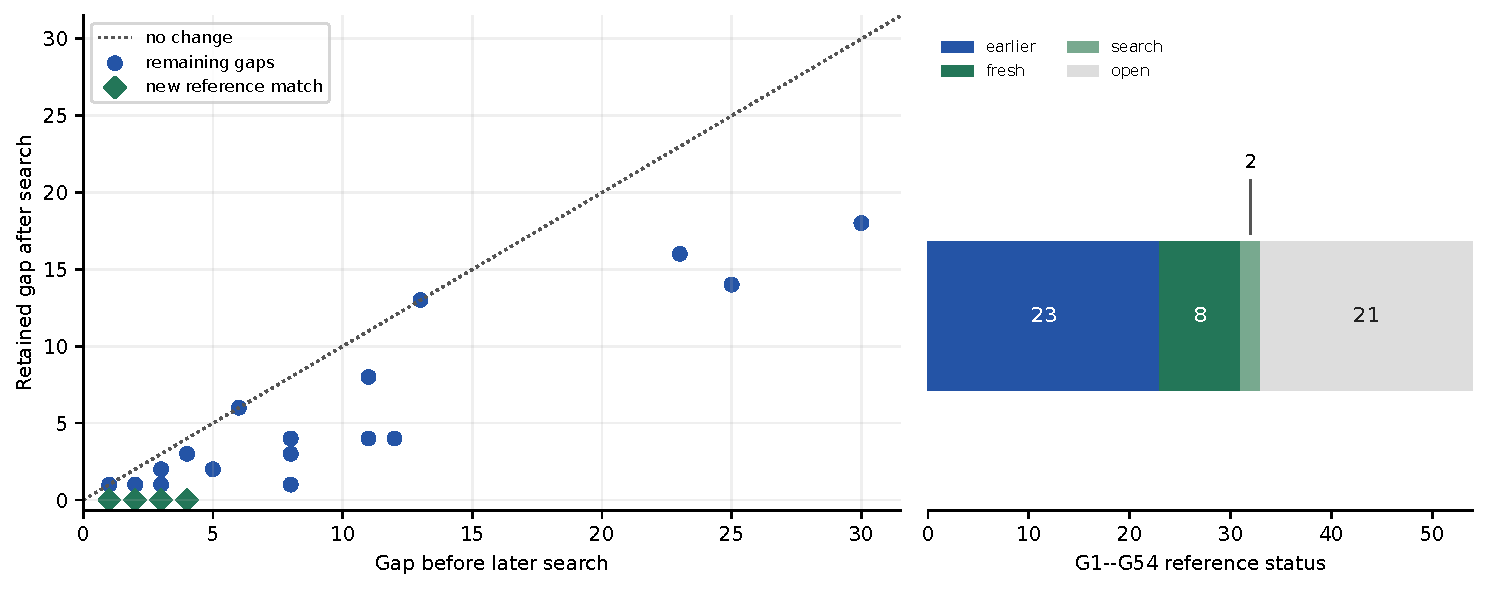
\includegraphics[width=\textwidth]{figures/gset_search_progress.pdf}
\caption{\textbf{Targeted \QeFEM{} updates extend
attainment on previously unresolved graphs.} Each point in the left panel
is one of the 31 graphs below its supplied reference before the later
search. Points below the diagonal improved; diamonds on the horizontal
axis are the ten new matches. The right panel separates the accumulated
54-graph inventory into 23 prior matches, eight new matches recovered
with fresh seeds, two found only during search, and 21 unmatched graphs.
Search budgets were adaptive, so the stacked bar is an attainment record,
not a universal success rate.}
\label{fig:gset-progress}
\end{figure*}

The improvements extend beyond the ten new matches. Most revisited
graphs move closer to their references even without reaching them. The
remaining failures are also concentrated: G14, G29, G30, G31, and G51
are one cut unit below their stored targets; G23, G26, and G40 are two
units below. The largest residuals are on G35--G38, with gaps 13, 16,
18, and 14 respectively. Appendix~\ref{app:fullresults} lists every
G1--G54 target, attained cut, gap, and evidence status. The 33 matches
do not establish an equal-budget advantage over another solver because
the cumulative search incorporated multiple graph-specific proposals.

\subsection{K2000: a strong cut, a population plateau, and an open gap}

K2000 tests a dense signed objective with nearly two million couplings.
The five frozen 8,192-replica \QeFEM{} trials yield cuts 33,274,
33,274, 33,274, 33,293, and 33,291. Their mean is 33,281.2 and sample
standard deviation is 9.88 cut units. The best cut is 44 below the
stored 33,337 reference, a residual of 0.132\% relative to that
reference. The corresponding five \LQA{} endpoints all equal 33,249,
giving gap 88. The smaller \QeFEM{} gap is an attainable-quality result
under these frozen method settings; it is not a matched-time win because
one \QeFEM{} trial evolves 8,192 states and one \LQA{} trial evolves one.

\begin{table*}[t]
\centering\small
\caption{All five frozen K2000 trials. The paired rows share a seed label;
the algorithms use different state representations and random-input
shapes. Both methods are rescored on the same raw graph.}
\label{tab:k2000trials}
\begin{tabular*}{\textwidth}{@{\extracolsep{\fill}}rrrrrr}
\toprule
trial & seed & \QeFEM{} cut & gap & \LQA{} cut & gap\\
\midrule
1 & 3371835386 & 33274 & 63 & 33249 & 88 \\
2 & 3700479728 & 33274 & 63 & 33249 & 88 \\
3 & 1934420243 & 33274 & 63 & 33249 & 88 \\
4 & 716463040 & 33293 & 44 & 33249 & 88 \\
5 & 424211264 & 33291 & 46 & 33249 & 88 \\
\bottomrule

\end{tabular*}
\end{table*}

The nested population study diagnoses how much of the gain comes from
additional initial conditions. At 128 replicas, the mean cut over five
seeds is 33,252 and the best is 33,255. At 2,048 replicas, these rise
to 33,272.6 and 33,293. Increasing the population further to 8,192
raises the mean to 33,281.2 but leaves the best at 33,293. Thus more
replicas improved average trial quality within the explored range, while
four times as many replicas after 2,048 did not close the final best-cut
gap. Figure~\ref{fig:k2000-population} makes both facts visible.

\begin{figure*}[t]
\centering
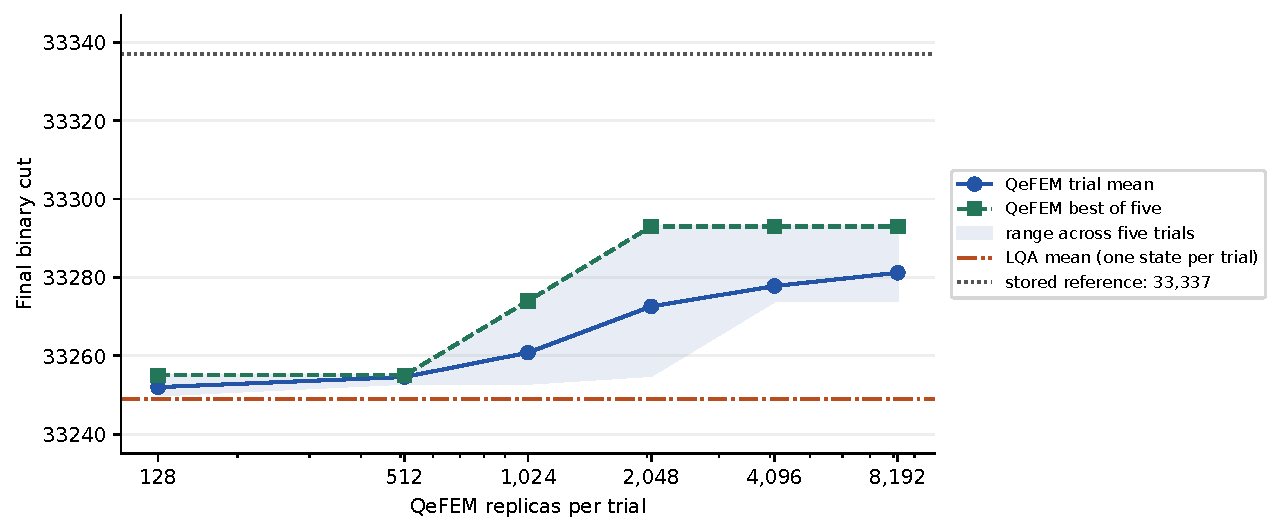
\includegraphics[width=.92\textwidth]{figures/k2000_population.pdf}
\caption{\textbf{Population search improves K2000 cut quality,
with diminishing best-cut returns.} QeFEM's mean, range, and best final
cut across five paired seeds are shown at each nested population size.
The saved \LQA{} mean (one state per trial) and the 33,337 stored target
are horizontal references. The best \QeFEM{} cut rises from 33,255
at 128 replicas to 33,293 by 2,048, then remains there through 8,192.
No point in this figure implies a matched-compute comparison.}
\label{fig:k2000-population}
\end{figure*}

The coherent final-winner trajectory in Fig.~\ref{fig:k2000-dynamics}
provides an additional view of the search. Its discrete reference gap
falls by orders of magnitude over the run, while local entropy per spin
decreases overall. The early entropy dip and rebound show that neither
entropy nor discrete cut changes monotonically under RMSprop and a
changing objective. The driver reaches zero halfway; the final portion
continues to refine the same candidate under a classical objective.
This selected trajectory illustrates a mechanism visible in one successful
trial; it does not describe the distribution of all 8,192 replicas.

\begin{figure*}[t]
\centering
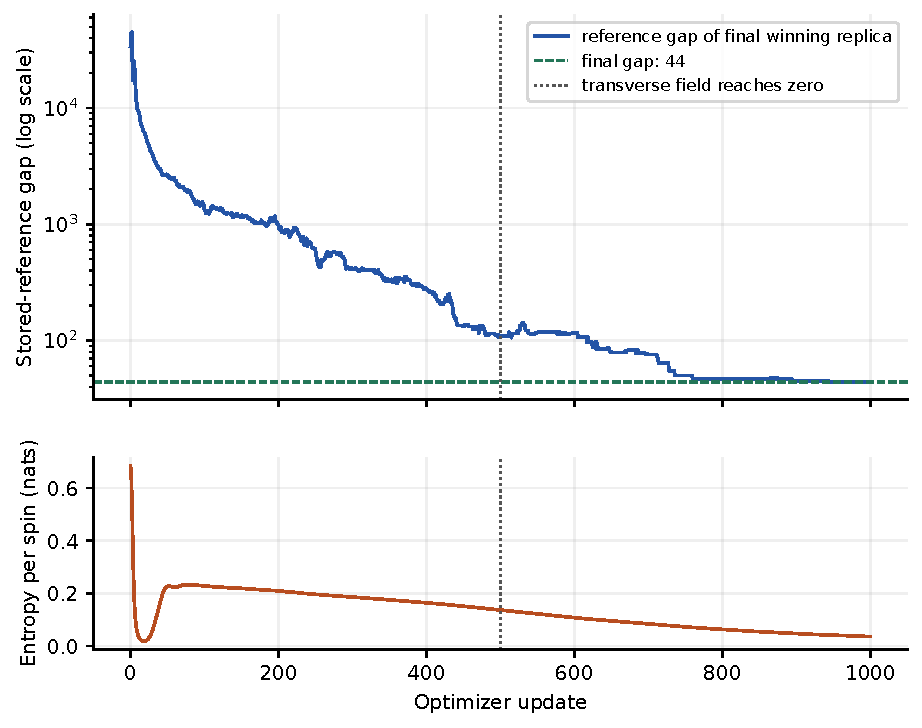
\includegraphics[width=.86\textwidth]{figures/k2000_winner_dynamics.pdf}
\caption{\textbf{Annealed mixed-state optimization can turn a
poor initialization into a near-reference binary solution.} The upper
panel shows the stored-reference gap on a logarithmic scale for one
coherent replica: the final winner of the best 8,192-replica K2000 trial.
The lower panel shows its mean single-site entropy. The dotted vertical
line marks the end of the transverse-field schedule; the dashed
horizontal line marks the final gap of 44. This is one replica's replay,
not a per-step maximum over the population.}
\label{fig:k2000-dynamics}
\end{figure*}

Taken together, the K2000 results support a specific and bounded claim.
The frozen mixed-state solver produces a high cut and improves on the
saved one-state \LQA{} baseline, but the explored population scaling
does not reach the reference. A new schedule or the G-set discrete update
might change that outcome; neither has been evaluated here and neither
can be credited for the frozen K2000 result.

\subsection{Wishart: lower error on every fixed planted instance}

The Wishart mean relative energy error is 4.0717\% for \QeFEM{} and
6.9411\% for the saved \LQA{} comparator. The difference is 2.8693
percentage points, or a 41.3\% reduction relative to the latter mean.
\QeFEM{} has lower mean error at each of the ten requested $\alpha$
values. Exact planted-energy hits occur in two of five trials at
$\alpha=0.9$ and all five at $\alpha=1.0$; the saved \LQA{} runs have
none across the 50 trials. The late improvement of \QeFEM{} after a
larger error at $\alpha=0.8$ is consistent with an easy--hard--easy
pattern in this particular ten-file series, but these fixed files alone
do not estimate an ensemble-wide hardness curve
\citep{hamze2020}.

\subsection{Chook: a wide planted-hit region}

Across the eleven tile-planted files, \QeFEM{} has equal-instance mean
relative error 0.2186\%; the saved \LQA{} mean is 1.1086\%. The
absolute difference is 0.8900 percentage points, corresponding to an
80.3\% relative reduction. \QeFEM{} has lower mean error on every file.
It reaches the planted energy in all ten trials for every requested
$p(C_3)$ from 0.5 through 1.0, accounting for 60 of 110 trial hits.
\LQA{} has four hits at 0.9 and six at 1.0, for ten of 110 overall.
The requested $p(C_3)$ is a generator setting; the realized tile
fraction of a finite instance can differ slightly.

\begin{figure*}[t]
\centering
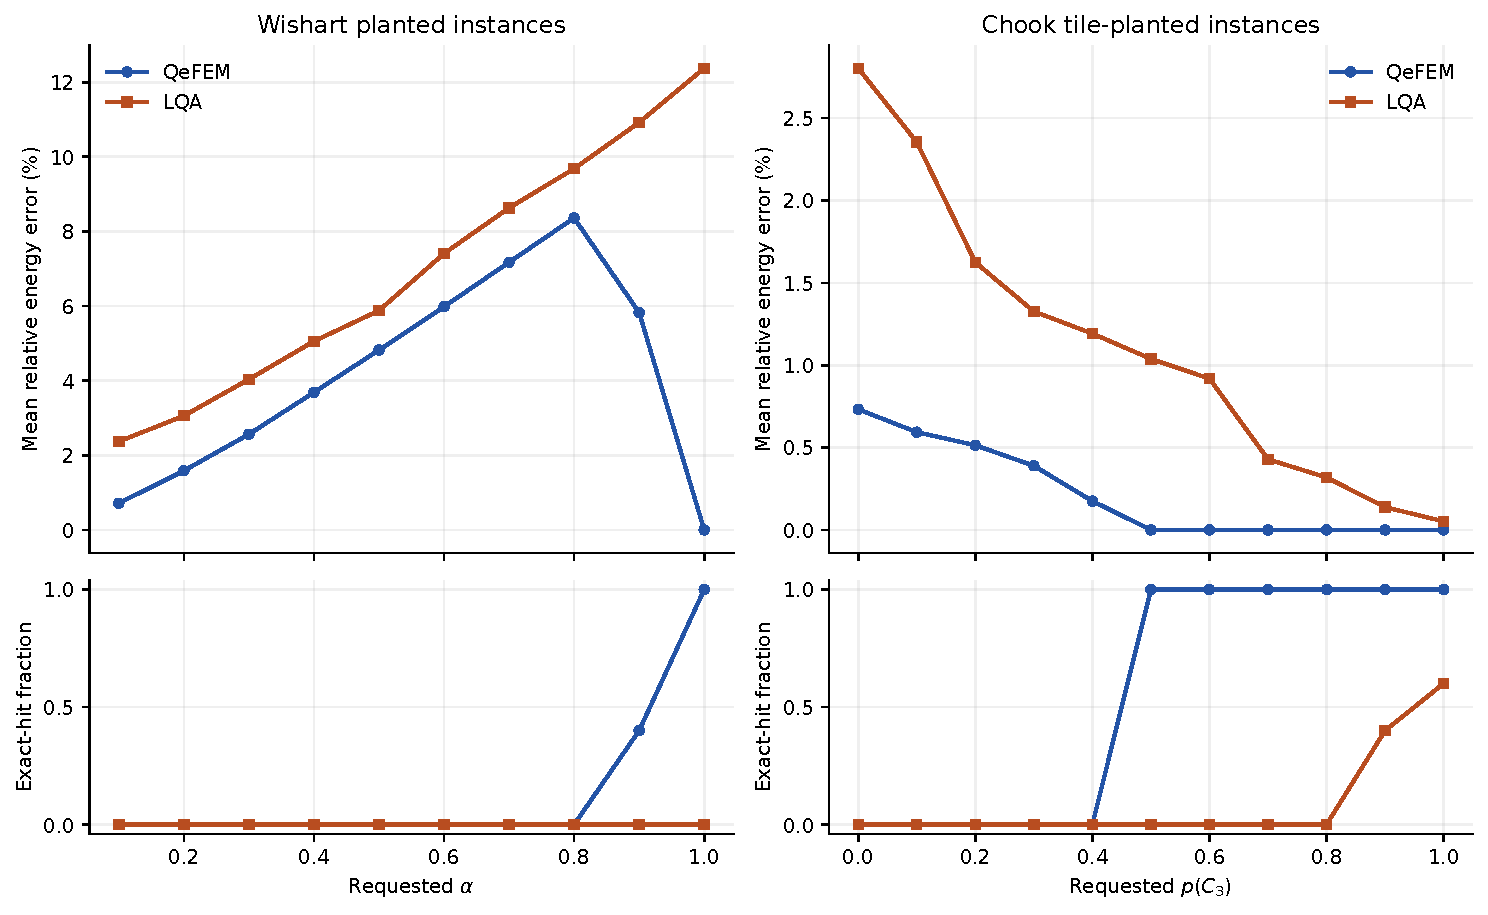
\includegraphics[width=\textwidth]{figures/planted_instance_errors.pdf}
\caption{\textbf{Under the saved configurations, \QeFEM{}
improves quality throughout both planted suites and reaches exact
solutions more often.} Top panels show trial-mean relative energy error
on each fixed Wishart and Chook instance. Bottom panels show the fraction
of trial populations whose best final replica has exactly the planted
energy. There are five trials per Wishart instance and ten per Chook
instance. The curves connect different fixed files and are visual guides,
not uncertainty bands or estimates over newly sampled instances.}
\label{fig:planted}
\end{figure*}

The two measures capture complementary outcomes. A lower mean error on
every file demonstrates consistent improvement over
the declared comparator, while exact hits distinguish a merely close
endpoint from a solved planted instance. The same plot also shows where
the gap has not closed: Wishart $\alpha\leq0.8$ yields no exact hit in
these five-seed batches.

\section{Discussion}
\label{sec:discussion}

\subsection{What the experiments establish}

The evidence identifies a useful algorithmic property: the same
factorized mixed-state construction produces competitive binary
assignments on sparse and dense MaxCut graphs and on two structurally
different planted Ising families. On the saved planted files, the
\QeFEM{} configuration has lower error than the declared \LQA{}
configuration in every instance, and it returns exact planted energies
in seven Wishart and 60 Chook trial populations. The G-set continuation
adds ten previously unattained reference cuts, eight of them recovered
with frozen settings on fresh seeds. These are concrete strengths, not
claims of quantum hardware advantage or universal optimality.

The dynamics help explain why those strengths are plausible. The
product-state expectation is cheap enough for a large replica batch;
high-temperature entropy gives a smooth starting regime; the driver
offers an additional local direction during part of the search; and
cooling lets the longitudinal coupling landscape determine the final
binary choices. Spectral scaling provides a principled coordinate for
the onset of longitudinal instability on zero-field graphs. None of
these mechanisms guarantees the best basin, but each gives a testable
design variable rather than an opaque postprocessing step.

The K2000 result imposes an equally clear boundary. A best cut of 33,293
is strong relative to the saved 33,249 \LQA{} cut, yet it remains 44
below the stored 33,337 reference. The best cut stops improving in the
recorded nested population sweep after 2,048 replicas. A larger
population alone therefore has no demonstrated route to reference
attainment in these data. The available \FEM{}/\dSB{} notebook outputs
reach 33,337 under their own protocols. The correct conclusion is that
the present \QeFEM{} K2000 configuration does not match those attained
cuts; the evidence does not establish that the state family is incapable
of matching them under a different schedule or update. Conversely,
theoretical inclusion of a classical endpoint does not prove a finite
\QeFEM{} run must outperform tuned \FEM{} dynamics. The endpoint
proposition in Sec.~\ref{sec:theory} makes that distinction exact.

\subsection{Why this can matter outside the present benchmarks}

Many scheduling, allocation, routing, and design tasks admit QUBO or
Ising formulations \citep{lucas2014}. Once such a formulation is
available, the variational state, entropy evaluation, readout, and
batch optimizer in \QeFEM{} do not depend on the application's name;
the objective enters through its fields and pair couplings. That
separation makes the method attractive for an optimization platform
that must support many binary models on accelerator hardware. The
experiments here support the \emph{technical possibility} of scaling a
single implementation from sparse G-set graphs to a 2,000-spin dense
graph and to planted suites with known targets. They do not yet measure
business value, deployment reliability, constraint satisfaction after
QUBO penalty tuning, or total energy and monetary cost on an industrial
workload. Those questions require application-specific experiments.

The distinction also shapes how performance should be communicated.
A result such as 60/110 planted-energy hits conveys something different
from an average percent error; together they show how often the method
fully solves a fixed file and how far the remaining runs miss. The
G-set count is compelling as an attainment inventory, but its adaptive
search budget must accompany it. On K2000, a 0.132\% reference-relative
residual sounds small, but the absolute 44-unit gap is the more direct
optimization fact on a signed-weight graph. Clear plots and complete
captions can present a strong algorithm without converting unlike
protocols into an unsupported ranking.

\subsection{Limitations and decisive next experiments}

The product ansatz omits intersite correlations and entanglement.
Low-temperature spin-glass landscapes can have many metastable basins,
and the optimizer follows a finite, schedule-dependent path rather than
the instantaneous variational minimum. The manual discrete-neighbour
update can further improve attainable cuts, but it is a surrogate
vector field, not the exact free-energy gradient. No general convergence
or approximation-ratio theorem is claimed for the complete practical
solver. In particular, an observed local spectral instability does not
imply global MaxCut optimality.

Several limitations are experimental. The plotted G-set total
accumulates adaptive tuning, historical runs, and fresh-seed
confirmation. K2000 has one graph and five canonical \QeFEM{} seeds;
the plotted planted series has one fixed file at each parameter.
Family-level hyperparameters were selected after exploration of related
data. The saved \LQA{} comparison evolves one state per trial, whereas
\QeFEM{} evolves 8,192, and its planted settings include a local driver
choice. No wall-clock-normalized or candidate-normalized ranking is
possible from these endpoints alone. Even the FEM/dSB K2000 notebook
is a contextual source rather than a matched three-way protocol; its
saved output predates a later device-selection code change, so the
exact numbers should be freshly reproduced before they become a formal
new head-to-head figure.

A decisive K2000 study would freeze graph input, precision, device,
scoring code, and a predeclared total-work budget across \QeFEM{},
\FEM{}, and \dSB{}. It would vary the \QeFEM{} schedule and the
G-set-derived manual-discrete update under separate, recorded
hyperparameter searches; then it would evaluate selected settings on
fresh seeds without moving the goalposts. Reporting per-replica cut
distributions, hit counts, time-to-target, and memory would determine
whether the remaining gap is a schedule issue, a basin-coverage issue,
or a more structural limitation. The current paper does not include
such a trial, and it does not extrapolate the G-set gains to K2000.

\section{Conclusion}

\QeFEM{} gives a mathematically explicit route from a binary Ising
objective to a differentiable, annealed search over local mixed states.
The quantum relative entropy supplies the free-energy principle; the
product ansatz makes it computationally tractable; the Bloch-field map
guarantees valid local states; and binary readout returns ordinary
feasible solutions. The theory locates a graph-dependent longitudinal
instability scale and shows exactly where the later discrete-neighbour
search departs from the smooth gradient.

Under the saved protocols, the method reaches 33 of 54 G-set reference
cuts across accumulated searches, improves the declared \LQA{}
comparison on every fixed Wishart and Chook instance, and gives a
33,293 K2000 cut while leaving a 44-unit reference gap. These results
make a coherent case for \QeFEM{} as a flexible classical optimization
framework with strong solution quality on several large binary
landscapes. They also identify the next falsifiable question: whether
the new search dynamics and carefully matched resources can close the
dense K2000 gap without relying on ever larger replica populations.

\section*{Author contributions}
R.D. conceived and developed the core \QeFEM{} method, implemented the
original solver, designed the analysis workflow, and drafted the
manuscript. F.P. contributed the nonlinear reparameterization,
optimizer and schedule refinement, and benchmark testing. Both authors
interpreted the results and take responsibility for the final text.


\clearpage
\bibliographystyle{apsrev4-2}
\bibliography{references}

\onecolumngrid
\appendix
\section{Detailed derivations and limiting cases}
\label{app:derivations}

\subsection{From quantum relative entropy to a product free energy}

The Gibbs target of Eq.~\eqref{eq:gibbs} is full rank for $T>0$. Starting
from the definition of relative entropy,
\begin{align}
 \KL(\rho\Vert\sigma_{T,\Gamma})
 &=\Tr(\rho\log\rho)-\Tr(\rho\log\sigma_{T,\Gamma})\nonumber\\
 &=-S(\rho)+\frac{\Tr(\rho H_\Gamma)}{T}
                 +\log Z_{T,\Gamma}.
 \label{eq:app-kl}
\end{align}
Multiplication by $T$ immediately gives Eq.~\eqref{eq:klidentity}.
The omitted constant in an optimization is $-T\log Z$, which depends
on $(T,\Gamma)$ but not on the variational fields. Omitting it from
gradient calculations is valid even though its value changes along the
schedule. The exact Gibbs minimum is outside the factorized family in
general, so the restricted minimum only bounds the exact free energy
from above.

For a product state $\rho=\bigotimes_i\rho_i$, the logarithm separates
as $\log\rho=\sum_i I\otimes\cdots\otimes\log\rho_i\otimes\cdots\otimes I$,
giving $S(\rho)=\sum_iS(\rho_i)$. For $i\ne j$,
\begin{equation}
 \Tr[\rho(Z_iZ_j)]
 =\Tr(\rho_iZ_i)\Tr(\rho_jZ_j)=m_{z,i}m_{z,j}.
 \label{eq:app-factor}
\end{equation}
The transverse expectation is $\Tr(\rho X_i)=m_{x,i}$. These identities
give Eq.~\eqref{eq:qefemF} without sampling any spin configuration.

\subsection{The local state, entropy, and field map}

Let $A_i=u_iX_i+v_iZ_i$. The Pauli anticommutation relation gives
$A_i^2=(u_i^2+v_i^2)I=r_i^2I$. Separating even and odd terms of the
exponential series,
\begin{equation}
 e^{A_i}=\cosh r_i\,I+
           \frac{\sinh r_i}{r_i}A_i.
 \label{eq:app-exp}
\end{equation}
Dividing by $\Tr e^{A_i}=2\cosh r_i$ produces
$\rho_i=\tfrac12[I+(\tanh r_i/r_i)A_i]$. Thus the Bloch radius is
$R_i=\tanh r_i$, and the eigenvalues are $(1\pm R_i)/2$.
Substituting those eigenvalues into $-\Tr\rho_i\log\rho_i$ yields
Eq.~\eqref{eq:entropy}. Alternatively, from
$\log\rho_i=A_i-\log(2\cosh r_i)I$,
\begin{align}
 S_i&=-\Tr(\rho_i A_i)+\log(2\cosh r_i)\nonumber\\
    &=\log(2\cosh r_i)-r_i\tanh r_i,
 \label{eq:app-entropy}
\end{align}
because $\Tr(\rho_i A_i)=r_iR_i$.

The apparent singularity at $r=0$ in $g(r)=\tanh r/r$ is removable.
Expanding $\tanh r$ around zero gives
\begin{equation}
 g(r)=1-\frac{r^2}{3}+\frac{2r^4}{15}+O(r^6),
 \qquad
 \operatorname{sech}^2r=1-r^2+\frac{2r^4}{3}+O(r^6).
 \label{eq:app-series}
\end{equation}
These limits justify a smooth origin and the numerical safe branch in
the implementation.

\subsection{Gradient and Hessian in physical and field coordinates}

Writing $\bm m=(m_x,m_z)$ and $R=\|\bm m\|$, the scalar derivative of
Eq.~\eqref{eq:entropy} is
\begin{equation}
 \frac{dS}{dR}
 =-\frac12\log\frac{1+R}{1-R}
 =-\operatorname{arctanh}R.
 \label{eq:app-ds}
\end{equation}
As $\nabla_{\bm m}R=\bm m/R$ away from the origin,
$\nabla_{\bm m}(-TS)=T\operatorname{arctanh}R\,\bm m/R$.
Adding the problem and driver gradients gives
Eqs.~\eqref{eq:gradx}--\eqref{eq:gradz}. To move to unconstrained
fields, differentiate $\bm m=g(r)\bm a$:
\begin{equation}
 d\bm m=g(r)d\bm a+
   g'(r)\bm a\frac{\bm a^{\mathsf T}d\bm a}{r}.
 \label{eq:app-dm}
\end{equation}
This is Eq.~\eqref{eq:jacobian}. In the radial direction
$\bm a/r$, the Jacobian eigenvalue is
$g(r)+rg'(r)=d(\tanh r)/dr=\operatorname{sech}^2r$;
in every tangential direction it is $g(r)$. Since
$J\bm a=\operatorname{sech}^2r\,\bm a$,
the chain rule applied to Eq.~\eqref{eq:physicalgrad} gives
Eq.~\eqref{eq:fieldgrad}. No derivative of a sign function appears in
this exact smooth calculation.

For completeness, the physical-coordinate Hessian of the negative
single-site entropy has the radial and tangential eigenvalues
\begin{equation}
 \lambda_{\rm rad}=\frac{1}{1-R^2},
 \qquad
 \lambda_{\rm tan}=\frac{\operatorname{arctanh}R}{R}.
 \label{eq:app-entropy-hessian}
\end{equation}
They follow by differentiating the radial vector field
$\nabla(-S)=(\operatorname{arctanh}R/R)\bm m$. Since
$\operatorname{arctanh}R\geq R$ for $0\leq R<1$, both are at least one.
The graph contribution to the Hessian acts only on longitudinal
coordinates and equals $K$. Thus $T> -\lambda_{\min}(K)$ is a sufficient
condition for strict convexity of the physical-coordinate objective.
This does not imply convexity in the nonlinear field coordinates
$\bm a$; reparameterization may change curvature even while preserving
finite-field stationary points.

\subsection{Longitudinal instability and spectral schedule inversion}

When $h=0$ and $\bm m_z=0$, the stationary local $x$ component is
$m_x=\tanh(\Gamma/T)$. The graph term has quadratic expansion
$\tfrac12\bm m_z^{\mathsf T}K\bm m_z$. Holding the stationary transverse
component fixed for a longitudinal perturbation, the local entropy
curvature contributes
\begin{equation}
 T\frac{\operatorname{arctanh}m_x}{m_x}
 =\frac{\Gamma}{\tanh(\Gamma/T)}=q(T,\Gamma).
 \label{eq:app-q}
\end{equation}
The mixed $x$--$z$ Hessian vanishes at $m_z=0$ by symmetry, so
Eq.~\eqref{eq:stability} is also the relevant longitudinal block of
the full Hessian. If the lowest eigenvalue of $K$ is $-\kappa$, the
quadratic form first loses positive definiteness at $q=\kappa$.
Setting $\rho=\Gamma/T$ gives
$q=T\rho/\tanh\rho$. Algebraic inversion yields
$T=q\tanh\rho/\rho$ and $\Gamma=q\tanh\rho$, as used in the
graph-specific G-set schedule. The stability calculation assumes zero
local fields and concerns a local stationary solution; it is not a
global approximation guarantee.

\subsection{Quadratization example and its penalty requirement}

The formal reach of a QUBO solver extends to higher-order binary terms
when auxiliary variables are introduced, although that extension is not
benchmarked here. For $x,y,z\in\{0,1\}$, the penalty
\begin{equation}
 P\bigl(xy-2xz-2yz+3z\bigr),\qquad P>0,
 \label{eq:app-quadratize}
\end{equation}
is zero when $z=xy$ and strictly positive for the other assignments.
For example, $(x,y)=(0,0)$ gives penalty $3Pz$;
$(1,0)$ or $(0,1)$ gives $Pz$; and $(1,1)$ gives $P(1-z)$.
To preserve the optimum of a surrounding objective, $P$ must exceed
the maximum possible improvement gained by violating the intended
relation. Repeated substitutions can increase variable count and
coefficient spread. Consequently QUBO encodability alone is not a
performance claim for a new application.

\section{Protocol, source, and comparator details}
\label{app:protocols}

\subsection{Exact saved-plan provenance}

The canonical K2000, Wishart, and Chook configurations are read from
the following frozen plan files in the companion \texttt{qefem\_prof}
repository:
\begingroup\footnotesize
\begin{itemize}[leftmargin=2em]
 \item \path{benchmarks/k2000/results/portable_accuracy_recheck/final_k2000/plan.json};
 \item \path{benchmarks/wishart/results/portable_accuracy_recheck/final_wishart/plan.json};
 \item \path{benchmarks/chunk/results/portable_accuracy_recheck/final_chook_a/plan.json}
       and \path{final_chook_b/plan.json}.
\end{itemize}
\endgroup
The paper workspace retains the parsed configurations and endpoint rows
under \path{Paper/results/}. It records the Python, NumPy, and PyTorch
versions, the numerical device, dtype, input hashes, and the declared
source revision in \path{results/experiment_environment.json} and the
case-level configuration and manifest files. The frozen K2000
\QeFEM{} job was selected from \path{scale_k2000/momentum_fast}.
That selection predates the later G-set manual-discrete search. No
G-set spectral or discrete-neighbour setting was silently transferred
to the plotted K2000 results.

Each K2000 seed is obtained from the declared base seed 50,000 by the
repository's deterministic derivation function. The resulting five
seed values are listed in Table~\ref{tab:k2000trials}; the LQA rows
share those labels. Wishart and Chook likewise retain their exact seed
arrays in each instance's \path{configuration.json}. A seed controls
initial pseudo-random fields, not the quality of the optimum itself.
Different algorithms map the same integer to different state shapes,
so a shared label is useful for auditing but not a proof of paired
random trajectories.

\subsection{The G-set search variants}

The smooth G-set stage used a product-state objective with exact
automatic differentiation. The later remaining-gap search used both
an exact manual evaluation of Eq.~\eqref{eq:fieldgrad} and the
surrogate direction of Eq.~\eqref{eq:discretenbr}. Its spectral schedule
computes $\kappa$ from the smallest eigenvalue of the normalized graph
coupling matrix, constructs a decreasing $q/\kappa$ curve, and chooses a
decreasing ratio $\rho=\Gamma/T$. Equation~\eqref{eq:spectralinvert}
then generates the temperature and driver arrays. Most transferred
discrete-update proposals used SGD with momentum 0.95 and weight decay
0.01; exact proposals retained their previous optimizer. This is a
graph-specific search, not one fixed set of hyperparameters across
all G-set graphs.

For the discrete mode, $\lambda_t$ can increase linearly between
declared start and end fractions or switch abruptly when those
fractions are equal. The implementation changes only the neighbor
magnetizations inside $K\widetilde{\bm m}_z$ and leaves the local
Bloch Jacobian and entropy contribution continuous. The final
configuration is always decoded and rescored against the original
graph. The full controller, per-graph plan, proposal registry, and
rescore audit are saved under
\path{benchmarks/Gset/results/remaining_discrete/}; its completed
analysis is the source of the 54-instance table in
Appendix~\ref{app:fullresults}.

\subsection{How the FEM and dSB context was handled}

The accompanying FEM repository contains a K2000 notebook with saved
cell output for separate \FEM{} and \dSB{} sweeps. The current notebook
source sets 1,000 replicas for each method and nominal update budgets
from 100 through 100,000. Its saved output reports the best cuts in
Table~\ref{tab:archived-context}. These values are included so the
reader can see that the current \QeFEM{} gap is a real competitive
limitation, not because the notebook is a controlled three-way trial.
The notebook itself states that its saved outputs predate a later
device-selection code update; rerunning is needed to align saved
values with the current MPS/CPU implementation. The published \FEM{}
paper reports its own K2000 protocol and figure
\citep{shen2025}; its figure should not be numerically identified with
this local notebook's later output.

\begin{table}[ht]
\centering\small
\caption{Selected best cuts printed by the archived FEM K2000 notebook,
with 1,000 FEM or dSB trajectories at each independent update budget.
These are contextual outputs, not matched comparisons with the separate
8,192-replica, five-trial QeFEM CPU evaluation. The stored reference is
33,337.}
\label{tab:archived-context}
\begin{tabular*}{\textwidth}{@{\extracolsep{\fill}}rrr}
\toprule
updates & archived FEM best & archived dSB best\\
\midrule
100 & 33,133 & 32,993\\
200 & 33,214 & 33,155\\
400 & 33,275 & 33,248\\
600 & 33,296 & 33,285\\
800 & 33,296 & 33,272\\
1,000 & 33,306 & 33,304\\
2,000 & 33,332 & 33,333\\
4,000 & 33,337 & 33,337\\
\bottomrule
\end{tabular*}
\end{table}

The FEM notebook uses RMSprop-like momentum settings
$\eta=0.03$, $\alpha=0.56$, momentum $0.63$, weight decay $0.013$,
$T_{\max}=1.16$, $T_{\min}=6\times10^{-5}$, and a graph-dependent
normalization in its classical FEM implementation. Its dSB implementation
uses step size $\Delta t=1.25$ and a sign-dependent coupling in a
position--momentum update. These are genuine algorithmic and protocol
differences. Figure~\ref{fig:k2000-population} consequently compares
only the frozen QeFEM population study with its explicitly declared
saved LQA baseline; it does not mix a FEM/dSB sweep into one curve.

\subsection{Figure data and rebuild command}

All four figures in this manuscript are generated by
\path{detailed/make_figures.py}. The script performs read-only loads of
saved endpoint, trajectory, and G-set analysis files; it executes no
optimizer. It writes vector PDF and PNG copies to
\path{detailed/figures/}, exact plot-ready aggregates to
\path{detailed/plot_data/}, and result-table rows to
\path{detailed/tables/}. The script asserts the expected K2000 five-seed
population counts and G-set 54-instance status total before plotting.
The figure captions identify whether they show a five-seed endpoint
summary, one coherent trajectory, fixed planted-instance means, or an
adaptive attainment inventory. Those distinctions are part of the
figure data, not small-print exceptions.

\section{Complete numerical tables}
\label{app:fullresults}

\subsection{Nested K2000 population sweep}

Table~\ref{tab:k2000-pop-all} prints the values underlying
Fig.~\ref{fig:k2000-population}. The same five seed labels are used at
each population size, and smaller populations are prefixes of the
8,192 initial fields. The target is 33,337 and the saved \LQA{} mean
and best are both 33,249.

\begin{center}
\begin{minipage}{\textwidth}
\small
\captionof{table}{K2000 QeFEM endpoint cuts over five seeds at each nested
population size. The best-gap column is relative to the stored 33,337
reference.}
\label{tab:k2000-pop-all}
\begin{tabular*}{\textwidth}{@{\extracolsep{\fill}}rrrr}
\toprule
replicas & mean cut & best cut & best gap\\
\midrule
128 & 33,252.0 & 33,255 & 82\\
512 & 33,254.6 & 33,255 & 82\\
1,024 & 33,260.8 & 33,274 & 63\\
2,048 & 33,272.6 & 33,293 & 44\\
4,096 & 33,277.8 & 33,293 & 44\\
8,192 & 33,281.2 & 33,293 & 44\\
\bottomrule
\end{tabular*}
\end{minipage}
\end{center}

\subsection{All fixed Wishart files}

\begin{center}
\begin{minipage}{\textwidth}
\small
\captionof{table}{Wishart results by requested $\alpha$. Each method has five
trial populations per fixed file. $\overline{\Delta E}$ is mean excess
over the supplied planted energy; $\overline\eps$ is mean relative
energy error. Hits count trial populations with an exact endpoint.}
\label{tab:wishart-all}
\centering
\begin{tabular}{crrrrrr}
\toprule
& \multicolumn{2}{c}{mean $\Delta E$}
& \multicolumn{2}{c}{mean $\eps$ (\%)}
& \multicolumn{2}{c}{exact hits}\\
$\alpha$ & QeFEM & LQA & QeFEM & LQA & QeFEM & LQA\\
\midrule
0.1 & 0.18 & 0.59 & 0.716 & 2.368 & 0/5 & 0/5 \\
0.2 & 0.79 & 1.53 & 1.586 & 3.059 & 0/5 & 0/5 \\
0.3 & 1.93 & 3.04 & 2.564 & 4.036 & 0/5 & 0/5 \\
0.4 & 3.70 & 5.08 & 3.687 & 5.057 & 0/5 & 0/5 \\
0.5 & 6.04 & 7.36 & 4.822 & 5.879 & 0/5 & 0/5 \\
0.6 & 8.98 & 11.11 & 5.983 & 7.408 & 0/5 & 0/5 \\
0.7 & 12.54 & 15.09 & 7.174 & 8.630 & 0/5 & 0/5 \\
0.8 & 16.66 & 19.30 & 8.360 & 9.681 & 0/5 & 0/5 \\
0.9 & 13.09 & 24.53 & 5.825 & 10.920 & 2/5 & 0/5 \\
1.0 & 0.00 & 30.95 & 0.000 & 12.373 & 5/5 & 0/5 \\
\bottomrule

\end{tabular}
\end{minipage}
\end{center}

\subsection{All fixed Chook tile-planted files}

\begin{center}
\begin{minipage}{\textwidth}
\small
\captionof{table}{Chook results by requested tile-mixture parameter $p(C_3)$.
Each method has ten trial populations per fixed file. Notation follows
Table~\ref{tab:wishart-all}.}
\label{tab:chook-all}
\centering
\begin{tabular}{crrrrrr}
\toprule
& \multicolumn{2}{c}{mean $\Delta E$}
& \multicolumn{2}{c}{mean $\eps$ (\%)}
& \multicolumn{2}{c}{exact hits}\\
$p(C_3)$ & QeFEM & LQA & QeFEM & LQA & QeFEM & LQA\\
\midrule
0.0 & 15.00 & 57.40 & 0.732 & 2.803 & 0/10 & 0/10 \\
0.1 & 11.80 & 46.80 & 0.594 & 2.354 & 0/10 & 0/10 \\
0.2 & 10.00 & 31.60 & 0.514 & 1.625 & 0/10 & 0/10 \\
0.3 & 7.40 & 25.20 & 0.389 & 1.326 & 0/10 & 0/10 \\
0.4 & 3.20 & 21.80 & 0.175 & 1.192 & 0/10 & 0/10 \\
0.5 & 0.00 & 18.60 & 0.000 & 1.039 & 10/10 & 0/10 \\
0.6 & 0.00 & 15.80 & 0.000 & 0.919 & 10/10 & 0/10 \\
0.7 & 0.00 & 7.20 & 0.000 & 0.429 & 10/10 & 0/10 \\
0.8 & 0.00 & 5.20 & 0.000 & 0.318 & 10/10 & 0/10 \\
0.9 & 0.00 & 2.20 & 0.000 & 0.138 & 10/10 & 4/10 \\
1.0 & 0.00 & 0.80 & 0.000 & 0.052 & 10/10 & 6/10 \\
\bottomrule

\end{tabular}
\end{minipage}
\end{center}

\subsection{Every G1--G54 retained cut}

The status labels below have strict provenance meanings. ``Prior'' means
the supplied reference had already been attained before the later
31-graph search. ``Fresh'' means a new match was recovered by the
frozen selected setting on fresh evaluation seeds. ``Search'' means a
new match was seen during discovery or promotion but not recovered
on its fresh seeds. ``Open'' means no saved result attained the
supplied reference. These are evidence labels, not intrinsic classes
of graph difficulty.

\begin{center}
\begin{minipage}{\textwidth}
\footnotesize
\setlength{\tabcolsep}{3.5pt}
\captionof{table}{Complete retained G1--G54 results from the accumulated search.
Targets are the supplied benchmark references, not certificates of
global optimality. The two blocks continue the same table.}
\label{tab:gset-all}
\begin{tabular*}{\textwidth}{@{\extracolsep{\fill}}lrrrl@{\hspace{18pt}}lrrrl}
\toprule
graph & ref. & best & gap & evidence &
graph & ref. & best & gap & evidence\\
\midrule
G1 & 11624 & 11624 & 0 & prior & G28 & 3298 & 3298 & 0 & search \\
G2 & 11620 & 11620 & 0 & prior & G29 & 3405 & 3404 & 1 & open \\
G3 & 11622 & 11622 & 0 & prior & G30 & 3413 & 3412 & 1 & open \\
G4 & 11646 & 11646 & 0 & prior & G31 & 3310 & 3309 & 1 & open \\
G5 & 11631 & 11631 & 0 & prior & G32 & 1410 & 1406 & 4 & open \\
G6 & 2178 & 2178 & 0 & prior & G33 & 1382 & 1376 & 6 & open \\
G7 & 2006 & 2006 & 0 & prior & G34 & 1384 & 1378 & 6 & open \\
G8 & 2005 & 2005 & 0 & prior & G35 & 7687 & 7674 & 13 & open \\
G9 & 2054 & 2054 & 0 & prior & G36 & 7680 & 7664 & 16 & open \\
G10 & 2000 & 2000 & 0 & prior & G37 & 7691 & 7673 & 18 & open \\
G11 & 564 & 564 & 0 & prior & G38 & 7688 & 7674 & 14 & open \\
G12 & 556 & 556 & 0 & prior & G39 & 2408 & 2404 & 4 & open \\
G13 & 582 & 582 & 0 & prior & G40 & 2400 & 2398 & 2 & open \\
G14 & 3064 & 3063 & 1 & open & G41 & 2405 & 2402 & 3 & open \\
G15 & 3050 & 3050 & 0 & fresh & G42 & 2481 & 2473 & 8 & open \\
G16 & 3052 & 3052 & 0 & fresh & G43 & 6660 & 6660 & 0 & prior \\
G17 & 3047 & 3047 & 0 & search & G44 & 6650 & 6650 & 0 & prior \\
G18 & 992 & 992 & 0 & fresh & G45 & 6654 & 6654 & 0 & prior \\
G19 & 906 & 906 & 0 & fresh & G46 & 6649 & 6649 & 0 & prior \\
G20 & 941 & 941 & 0 & prior & G47 & 6657 & 6657 & 0 & prior \\
G21 & 931 & 931 & 0 & fresh & G48 & 6000 & 6000 & 0 & prior \\
G22 & 13359 & 13359 & 0 & fresh & G49 & 6000 & 6000 & 0 & prior \\
G23 & 13344 & 13342 & 2 & open & G50 & 5880 & 5880 & 0 & prior \\
G24 & 13337 & 13337 & 0 & fresh & G51 & 3848 & 3847 & 1 & open \\
G25 & 13340 & 13340 & 0 & fresh & G52 & 3851 & 3848 & 3 & open \\
G26 & 13328 & 13326 & 2 & open & G53 & 3850 & 3846 & 4 & open \\
G27 & 3341 & 3341 & 0 & prior & G54 & 3852 & 3848 & 4 & open \\
\bottomrule

\end{tabular*}
\end{minipage}
\end{center}


\end{document}
